\section{Filtro pasabajos}

Se pidió aplicar a un filtro RC de frecuencia de corte $f_{0}=64\,(kHz)$
una onda cuadrada de $10\,V_{pp}$ con frecuencia de $f=32\,(kHz)$. Los resultados obtenidos empíricamente se muestran
en las figuras \ref{2_1} y \ref{2_4}. A su vez, se calculó la transferencia
ideal del circuito, resultando ser:

\begin{equation}
H(s)=\frac{1}{1+sRC}\label{eq:2_4}
\end{equation}

La simulación de la transferencia del circuito en LTSpice se ve en las figuras \ref{2_4} y \ref{2_5}.

\begin{figure}[H]
\begin{centering}
\includegraphics[scale=0.4]{../Ex2/resources2/scope_0} 
\par\end{centering}
\caption{Resultados}
\label{2_1} 
\end{figure}

\begin{figure}[H]
\begin{centering}
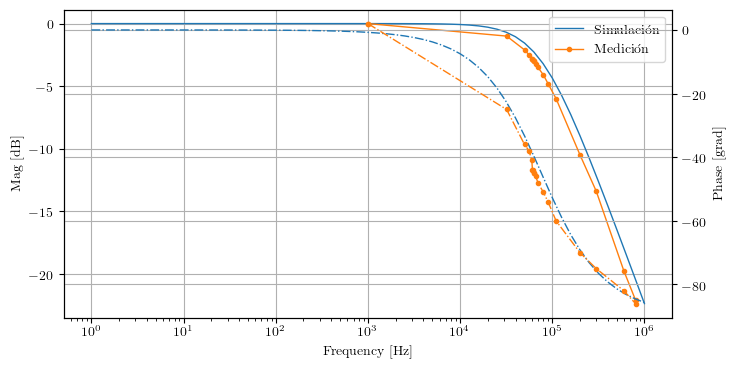
\includegraphics[scale=0.65]{../Ex2/resources2/MedyPost} 
\par\end{centering}
\caption{Simulación LTSpice y mediciones}
\label{2_4}
\end{figure}

\begin{figure}[H]
\begin{centering}
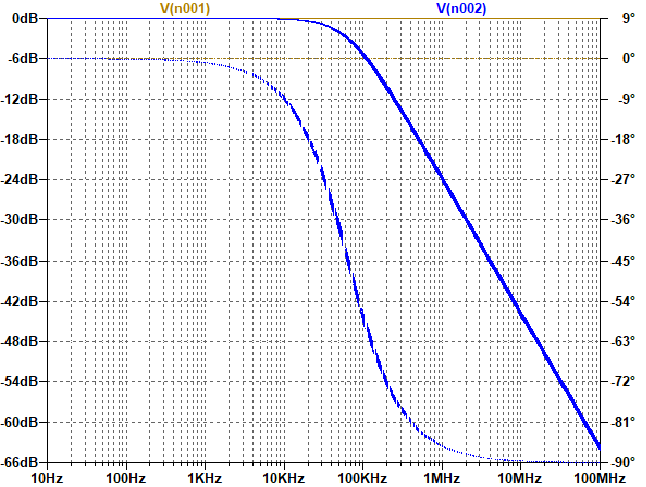
\includegraphics[scale=0.6]{../Ex2/resources2/montecarlo} 
\par\end{centering}
\caption{Análisis Montecarlo}
\label{2_5} 
\end{figure}

\subsection{Cálculo de armónicos}

Para estudiar la respuesta del circuito a una señal cuadrada, se debe
calcular primero cómo afecta el mismo a la onda de entrada.
Como sabemos que la onda es una cuadrada, haciendo su descomposición
en suma de señales trigonométricas los coeficientes de Fourier serán:

\[
a_{0}=0
\]

\[
a_{n}=0
\]

\[
b_{2n-1}=\frac{20}{(2n-1)\pi}
\]

\[
b_{2n}=0
\]

Por lo tanto, la entrada se puede expresar en el espacio temporal
como se ve en la fórmula \ref{eq:2_1}. Sin embargo,
por temas de idealización, una señal cuadrada ideal se puede
aproximar por una suma de términos finitos de senoidales:
si se aproxima la cuadrada con 10 términos, se puede ver cómo se va reduciendo el error. 
Esto se observa en la figura \ref{2_2}.

A medida que se agreguen más términos a la suma, menos será la
diferencia con una onda cuadrada ideal. No obstante, hay que tener
en cuenta que al tener una discontinuidad
no evitable cada $\frac{T}{2}$, siendo \emph{T} el período de la
señal, se generarán sobrepicos en los puntos de discontinuidad. Por
ende, si se llama \emph{x(t)} a la función cuadrada ideal e \emph{y(t)}
a su aproximación por senoides, \emph{x(t)} será igual a \emph{y(t)
}en todos los números reales exceptuando los puntos de discontinuidad.
Esto quiere decir que es posible que al trabajar con ondas cuadradas
se encuentren sobrepicos.

\begin{equation}
x(t)\sim\sum_{n=1}^{\infty}\frac{20}{(2n-1)\pi}sin\left(2\pi(2n-1)f_{0}t\right)\label{eq:2_1}
\end{equation}

\begin{figure}[H]
\begin{centering}
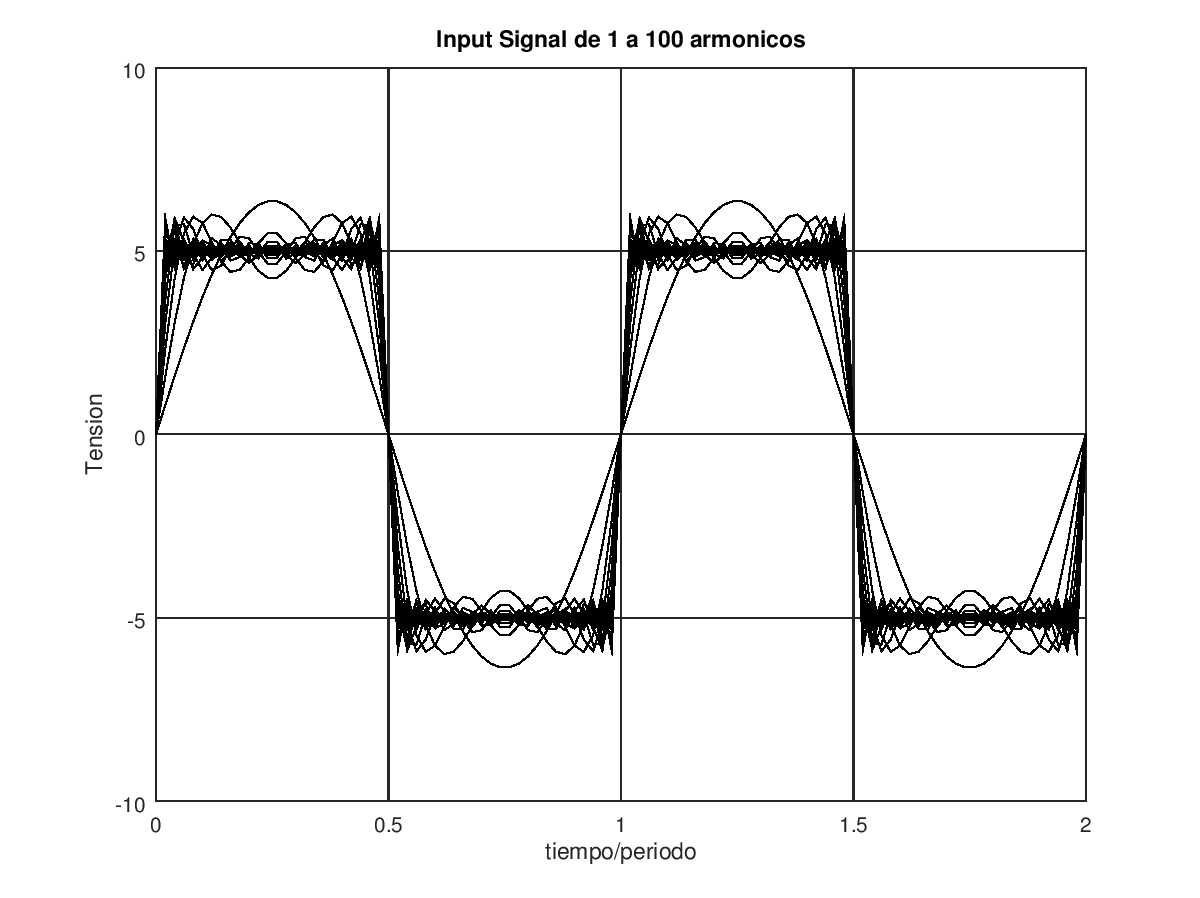
\includegraphics[scale=0.35]{../Ex2/resources2/Square}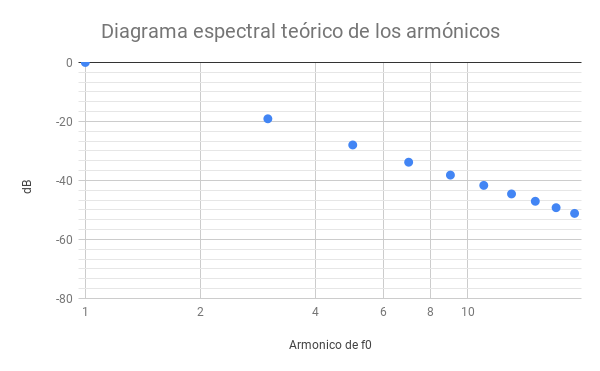
\includegraphics[scale=0.35]{../Ex2/resources2/DiagEspcTeo} 
\par\end{centering}
\caption{Representación de onda cuadrada mediante suma de senoidales y su diagrama
espectral teórico.}
\label{2_2} 
\end{figure}

\begin{figure}[H]
\begin{centering}
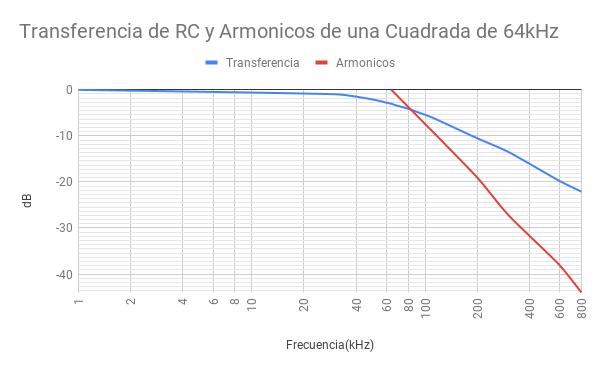
\includegraphics[scale=0.65]{../Ex2/resources2/Med_Arm} 
\par\end{centering}
\caption{Transferencia superpuesta con los armónicos (los puntos de los armónicos
están unidos por lineas)}
\end{figure}

Debido a que la entrada es una función continua a trozos de período
\emph{T, }

\[
y(t)\sim\sum_{n=1}^{\infty}\left|X_{2n-1}\right|\left|H\left((2n-1)f_{0}\right)\right|cos\left[2\pi(2n-1)f_{0}t+\phi((2n-1)f_{0})+\theta_{2n-1}\right]
\]

\begin{equation}
X_{2n-1}=i\frac{b_{2n-1}}{2}\label{eq:3}
\end{equation}

\[
H(f)=\left|H(f)\right|e^{i\phi(f)}
\]

A su vez,

\begin{equation}
H(f)=\frac{1}{1+i2\pi fRC}\label{eq:2}
\end{equation}

Por lo tanto, haciendo cálculos, de las ecuaciones \ref{eq:3} y \ref{eq:2},
se concluye que:

\[
\phi(f)=-arctg(2\pi fRC)
\]

\[
H(f)=\frac{1}{\sqrt{(2\pi fRC)^{2}+1}}
\]

\[
\theta_{n}=\frac{\pi}{2}
\]

Se puede escribir la salida como la ecuación \ref{eq:2_3}
y gráficamente se ve como la figura \ref{2_3}.

\begin{equation}
y(t)\sim\sum_{n=1}^{\infty}\frac{20}{(2n-1)\pi\sqrt{\left(2\pi(2n-1)f_{0}RC\right)^{2}+1}}cos\left(2\pi(2n-1)f_{0}t-arctg\left(2\pi(2n-1)f_{0}RC\right)+\frac{\pi}{2}\right)\label{eq:2_3}
\end{equation}

Teniendo en cuenta que $f_{0}=\frac{1}{2\pi RC}$ , y llamando \emph{k=2n-1,
}

\[
y(t)\sim\sum_{k\,impares}\frac{20}{k\pi\sqrt{k^{2}+1}}cos\left(2\pi kf_{0}t-arctg\left(k\right)+\frac{\pi}{2}\right)
\]

\begin{figure}[H]
\begin{centering}
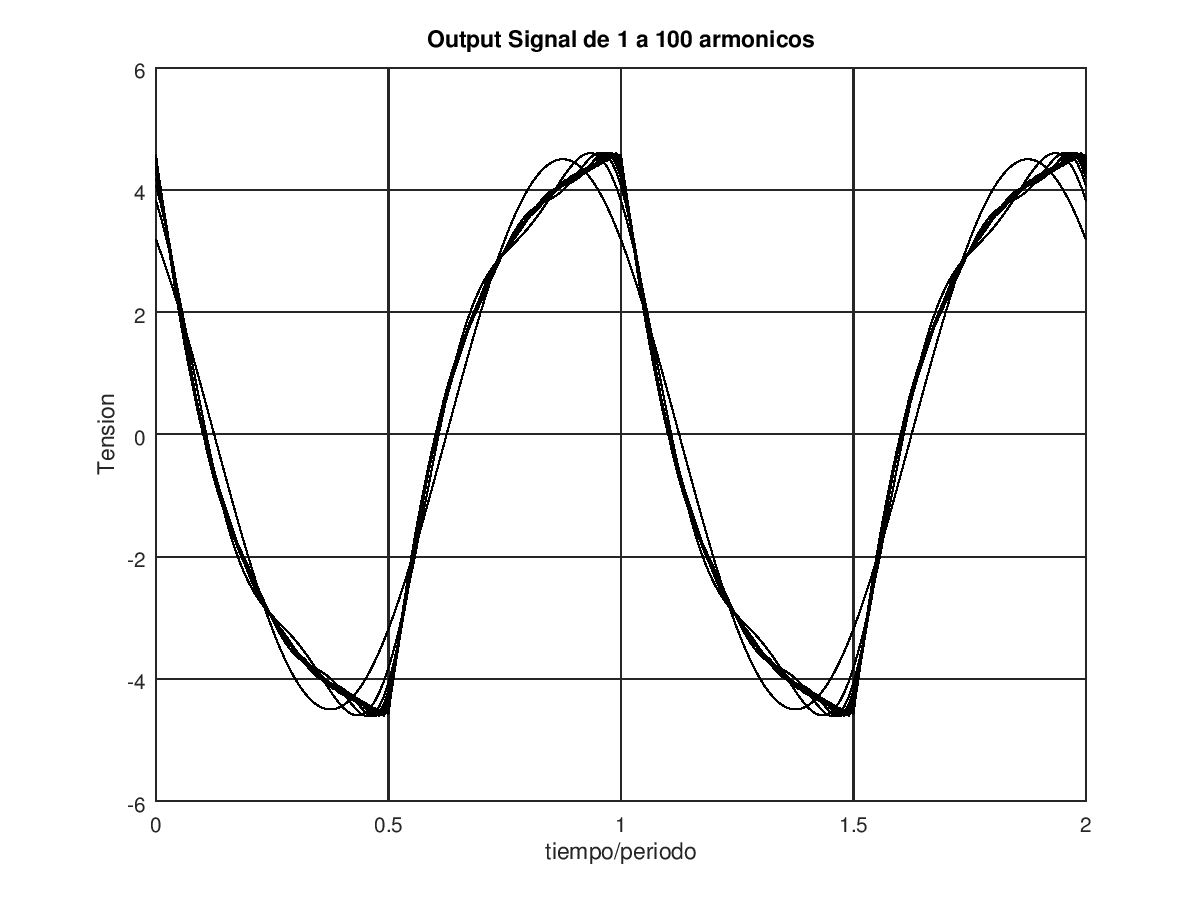
\includegraphics[scale=0.5]{../Ex2/resources2/out_calc} 
\par\end{centering}
\caption{Salida del RC en armónicos}
\label{2_3} 
\end{figure}

\subsection{Circuito como Integrador}

Un circuito integrador es aquel cuya
función transferencia es de la forma $H(s)=\frac{1}{s}$. Como se ve en la ecuación
\ref{eq:2_4}, el circuito estudiado no posee esa transferencia; sin embargo,
si se procura trabajar en un intervalo de frecuencias donde \emph{sRC }sea lo suficientemente
grande en comparación a la unidad, se puede aproximar la transferencia a la de un circuito integrador. Es decir:

\[
Si\,\,sRC\ggg1\Longrightarrow H(s)=\frac{1}{1+sRC}\approx\frac{1}{RC}\frac{1}{s}
\]

Por ende, si se cambia al espacio de frecuencias, procurando que $2\pi fRC\ggg1$
se puede obtener la transferencia de un circuito integrador. Si se eligen $R=3.68(k\Omega)\,y\,C=560(pF)$ se espera que para una
frecuencia $f_{a}\ggg63(kHz)$, el circuito se comporte como
un integrador.

En particular, si se tiene una frecuencia $f_{i}=300(kHz)$, se dará que $2\pi f_{a}RC\gg1$, con
lo cual podemos aproximar el denominador de la transferencia y usar
nuestro circuito como integrador, como se puede observar en la figura
\ref{2_6}.

\begin{figure}[H]
\begin{centering}
\includegraphics[scale=0.4]{../Ex2/resources2/300k} 
\par\end{centering}
\caption{Circuito como integrador a 300 (kHz)}
\label{2_6}
\end{figure}

\begin{figure}[H]
\begin{centering}
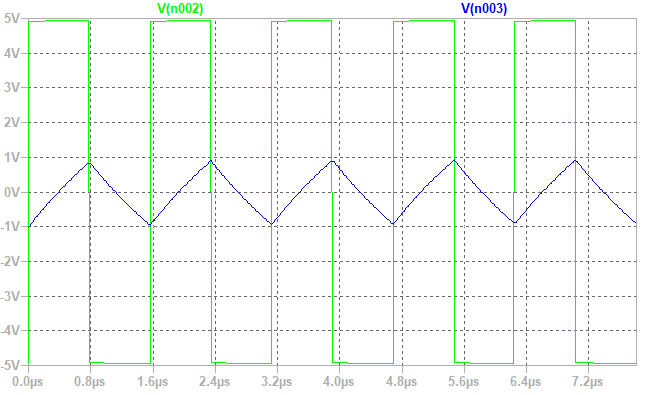
\includegraphics[scale=0.6]{../Ex2/resources2/sim} 
\par\end{centering}
\caption{Simulación del circuito a 300 (kHz)}
\end{figure}

\begin{figure}[H]
\begin{centering}
\includegraphics[scale=0.4]{../Ex2/resources2/640} 
\par\end{centering}
\caption{Circuito andando a 640(Hz)}
\end{figure}
